\documentclass[11pt]{article}
\usepackage[margin=1in]{geometry}
\usepackage{amsmath,amssymb,amsthm,graphicx,booktabs,xcolor,subcaption,enumitem,hyperref,caption}
\usepackage{algorithm}\usepackage{algpseudocode}
\captionsetup{font=small,labelfont=bf,skip=3pt}
\setlist{nosep,leftmargin=1.3em}
\setlength{\parskip}{2pt}
\newtheorem{theorem}{Theorem}
\graphicspath{{../figures/}}
% AUTO-GENERATED by report/make_tables.py from results/*.csv -- do not edit
\newcommand{\nInstTotal}{11{,}250}
\newcommand{\nRunsTotal}{225{,}000}
\newcommand{\nNonConv}{0}
\newcommand{\nA}{6,000}
\newcommand{\nV}{1,350}
\newcommand{\nL}{960}
\newcommand{\vOptMatch}{all}
\newcommand{\vMultiEq}{82}
\newcommand{\vMeanNash}{11}
\newcommand{\vMaxNash}{180}
\newcommand{\vPosEqPoa}{26}
\newcommand{\vSampledExact}{77}
\newcommand{\vOvershoot}{1.5}
\newcommand{\vPoaMean}{1.44}
\newcommand{\vPoaMax}{3.84}
\newcommand{\vPhiGap}{0.003}
\newcommand{\lossRhoZeroPFive}{0.18}
\newcommand{\lossRhoOnePZero}{0.23}
\newcommand{\lossRhoTwoPZero}{0.32}
\newcommand{\lossRhoFourPZero}{0.41}
\newcommand{\lossAlphaZeroPZero}{0.15}
\newcommand{\lossAlphaZeroPFive}{0.22}
\newcommand{\lossAlphaOnePZero}{0.31}
\newcommand{\lossAlphaOnePFive}{0.37}
\newcommand{\lossAlphaTwoPZero}{0.38}
\newcommand{\lossgrid}{0.26}
\newcommand{\losshubspoke}{0.31}
\newcommand{\lossscalefree}{0.29}
\newcommand{\hAlphaZeroPZero}{0.10}
\newcommand{\hAlphaZeroPFive}{0.12}
\newcommand{\hAlphaOnePZero}{0.18}
\newcommand{\hAlphaOnePFive}{0.30}
\newcommand{\hAlphaTwoPZero}{0.45}
\newcommand{\etaAlpha}{38}
\newcommand{\etaRho}{39}
\newcommand{\etaTopo}{1.8}
\newcommand{\lossTRgridZeroPFive}{0.18}
\newcommand{\lossTRgridOnePZero}{0.22}
\newcommand{\lossTRgridTwoPZero}{0.28}
\newcommand{\lossTRgridFourPZero}{0.36}
\newcommand{\lossTRhubspokeZeroPFive}{0.18}
\newcommand{\lossTRhubspokeOnePZero}{0.24}
\newcommand{\lossTRhubspokeTwoPZero}{0.37}
\newcommand{\lossTRhubspokeFourPZero}{0.45}
\newcommand{\lossTRscalefreeZeroPFive}{0.18}
\newcommand{\lossTRscalefreeOnePZero}{0.23}
\newcommand{\lossTRscalefreeTwoPZero}{0.32}
\newcommand{\lossTRscalefreeFourPZero}{0.41}
\newcommand{\lowRhoPeak}{0.29}
\newcommand{\lowRhoPeakAlpha}{1.5}
\newcommand{\lowRhoLast}{0.22}
\newcommand{\eqMaxLoadAlphaTwo}{10.6}
\newcommand{\optMaxLoadAlphaTwo}{1.3}
\newcommand{\eqCovAlphaTwo}{4.2}
\newcommand{\optCovAlphaTwo}{7.1}
\newcommand{\optIdleRhoFour}{72}
\newcommand{\eqIdleRhoFour}{13}
\newcommand{\olsRtwo}{0.69}
\newcommand{\kapPeak}{0.6}
\newcommand{\kapHubAtPeak}{0.37}
\newcommand{\kapGridAtPeak}{0.30}
\newcommand{\kapLowEnd}{0.26}
\newcommand{\kapHighEnd}{0.25}
\newcommand{\reguniformgrid}{0.05}
\newcommand{\regconcentratedgrid}{0.35}
\newcommand{\regdegreecorrelatedgrid}{0.09}
\newcommand{\reguniformhubspoke}{0.03}
\newcommand{\regconcentratedhubspoke}{0.36}
\newcommand{\regdegreecorrelatedhubspoke}{0.22}
\newcommand{\reguniformscalefree}{0.05}
\newcommand{\regconcentratedscalefree}{0.36}
\newcommand{\regdegreecorrelatedscalefree}{0.22}
\newcommand{\startRandom}{0.29}
\newcommand{\startDepot}{0.32}
\newcommand{\depotSpread}{0.000}
\newcommand{\lrnPlanMin}{0.98}
\newcommand{\lrnPlanCumMin}{0.8}
\newcommand{\lrnPlanCumMax}{8.5}
\newcommand{\lrnSelfCumUMin}{56}
\newcommand{\lrnSelfCumUMax}{87}
\newcommand{\lrnSelfCumGMin}{83}
\newcommand{\lrnSelfCumGMax}{115}
\newcommand{\lrnUcbBeatsFI}{87}
\newcommand{\lrnUcbGain}{+0.053}
\newcommand{\lrnGreedyGain}{-0.045}
\newcommand{\lrnRhoOneUcb}{0.76}
\newcommand{\lrnRhoOneFI}{0.69}
\newcommand{\eGiniEqLow}{0.09}
\newcommand{\eGiniOptLow}{0.36}
\newcommand{\eGiniEqHigh}{0.43}
\newcommand{\eGiniOptHigh}{0.85}
\newcommand{\eZeroOptHigh}{75}
\newcommand{\eZeroEqHigh}{13}
\newcommand{\eMoreUnequalAll}{93}
\newcommand{\eMoreUnequalDense}{100}
\newcommand{\eMoreUnequalSparse}{85}
\newcommand{\eUpdLow}{0.74}
\newcommand{\eUpdHigh}{1.10}
\newcommand{\eUpdMax}{1.38}
\newcommand{\eSweepsLow}{2.1}
\newcommand{\eSweepsHigh}{4.3}
\newcommand{\eSweepsMax}{7}
\newcommand{\nTests}{516}
\newcommand{\mutFail}{164}
\newcommand{\hungN}{900}
\newcommand{\hungDiff}{2.8\times10^{-14}}
\newcommand{\pilotMax}{29}
\newcommand{\lhFirst}{0.86}
\newcommand{\lhMid}{0.79}
\newcommand{\lhLast}{0.766}
\newcommand{\lhFI}{0.726}
\newcommand{\lhGain}{0.04}
\newcommand{\lhN}{30}
% AUTO-GENERATED by report/make_tables.py
\newcommand{\tabTopoRho}{\setlength{\tabcolsep}{3pt}\begin{tabular}{lcccc}\toprule
 & $\rho=0.5$ & $\rho=1$ & $\rho=2$ & $\rho=4$\\\midrule
Grid & 0.18 \scriptsize$\pm$0.01 & 0.22 \scriptsize$\pm$0.01 & 0.28 \scriptsize$\pm$0.01 & 0.36 \scriptsize$\pm$0.01\\
Hub-and-spoke & 0.18 \scriptsize$\pm$0.01 & 0.24 \scriptsize$\pm$0.01 & 0.37 \scriptsize$\pm$0.01 & 0.45 \scriptsize$\pm$0.01\\
Scale-free & 0.18 \scriptsize$\pm$0.01 & 0.23 \scriptsize$\pm$0.01 & 0.32 \scriptsize$\pm$0.01 & 0.41 \scriptsize$\pm$0.01\\
\bottomrule\end{tabular}}
\newcommand{\tabValidation}{\begin{tabular}{lr}\toprule Check (small instances, all equilibria enumerated) & Value\\\midrule
Instances & 1{,}350\\
Optimizer equals exhaustive optimum & all\\
Instances with more than one pure equilibrium & 82\%\\
Mean / max number of pure equilibria & 11 / 180\\
Best and worst equilibrium coincide (PoS = PoA) & 26\%\\
Sampled worst equals exact worst equilibrium & 77\%\\
Mean exact PoA / maximum & 1.44 / 3.84\\
Dynamics runs not converging (0 of 225{,}000) & 0\\
\bottomrule\end{tabular}}
\newcommand{\tabRegimes}{\setlength{\tabcolsep}{3pt}\begin{tabular}{lccc}\toprule Regime & Grid & Hub & Scale-free\\\midrule
Uniform & 0.05 & 0.03 & 0.05\\
Concentrated (80\% in 20\%) & 0.35 & 0.36 & 0.36\\
Degree-correlated & 0.09 & 0.22 & 0.22\\
\bottomrule\end{tabular}}
\newcommand{\tabLearning}{\begin{tabular}{lccccc}\toprule & \multicolumn{2}{c}{Coordinated} & \multicolumn{2}{c}{Selfish} & \\\cmidrule(lr){2-3}\cmidrule(lr){4-5}
$\rho$ & UCB & greedy & UCB & greedy & Selfish, full info\\\midrule
0.3 & 0.99 & 0.98 & 0.81 & 0.73 & 0.79\\
0.5 & 0.99 & 0.98 & 0.79 & 0.68 & 0.73\\
1 & 0.99 & 0.98 & 0.76 & 0.65 & 0.69\\
2 & 1.00 & 0.99 & 0.71 & 0.62 & 0.65\\
\bottomrule\end{tabular}}

\newcommand{\confirm}[1]{\textcolor{red}{#1}}
\newcommand{\Wopt}{W_{\mathrm{OPT}}}\newcommand{\Weq}{W_{\mathrm{EQ}}}
\hypersetup{colorlinks=true,linkcolor=blue!50!black,urlcolor=blue!50!black}
\title{\vspace{-1.2em}\textbf{How Much Does Selfishness Cost Taxi Drivers?}\\[2pt]
\large Efficiency of decentralized taxi positioning on stylized cities, and learning unknown demand\\[2pt]
\normalsize Foundations of AI and Multiagent Systems --- Final Project Report}
\author{Jahanzaib \and Mukkesh Dudekula \and Thushar Vunnam \and Lohith}
\date{}
\begin{document}\maketitle\vspace{-1.5em}
\begin{abstract}\noindent
Taxis choose where to wait for passengers. Left to themselves they crowd the profitable zones and leave others unserved; a dispatcher could do better. We model this as a congestion game with an idle option, prove it is an exact potential game (so best-response dynamics always converge), reduce the centralized optimum to a bipartite assignment, and measure the efficiency loss of selfish equilibria on \nInstTotal{} simulated instances over three city topologies, demand concentrations, driver densities and travel-cost scales. Driver density and demand concentration explain about \etaRho{}\% and \etaAlpha{}\% of the variance of the loss; the network topology only \etaTopo{}\%. Equilibrium welfare is lost because a driver who joins an occupied zone adds no demand but takes a share. In an extension where demand is unknown, learning costs a coordinating dispatcher under 3\% of welfare, while selfish drivers lose 19--38\% to selfishness itself; an exploration bonus even raises selfish efficiency by acting as an implicit subsidy to under-served zones.
\end{abstract}

\section{Problem and Changes from the Initial Idea}
\textbf{Decision problem.} $n$ taxi drivers each choose, every epoch, one of $m$ demand zones of a city graph (or to stay idle). Zones differ in how much fare revenue they generate; drivers differ in how far they must travel. We compare the \emph{selfish} outcome (a Nash equilibrium) with the \emph{coordinated} outcome (a dispatcher maximizing total welfare) and ask: \emph{how does the efficiency loss of selfish positioning depend on demand concentration, driver density, travel cost and city structure, and how does it change when demand is unknown and must be learned?}

\textbf{What changed since the idea review.} Table~\ref{tab:changes} lists every substantive change; most narrow the scope or sharpen a claim that the experiments forced us to revisit.
\begin{table}[!ht]\centering\footnotesize
\begin{tabular}{p{3.1cm}p{4.5cm}p{7.3cm}}\toprule
\textbf{Initial idea} & \textbf{Final project} & \textbf{Why}\\\midrule
Time-varying demand matched to real cities, classified from real metropolitan data & Static demand with a controlled concentration parameter on three stylized topologies & Isolates one factor at a time and keeps total demand fixed; real-city calibration was out of reach and would confound the sweep\\
Sequential mixed-strategy game, adversarial vs.\ cooperative & Repeated stage game with pure strategies: selfish (Nash) vs.\ coordinated (planner) & A pure equilibrium always exists (Thm.~\ref{thm:pot}); the planner is the cooperative benchmark\\
Utility = fares $-$ pickup $-$ trip cost $-$ idle penalty & $U_i=D(z)/n_z-\lambda c(\ell_i,z)$; idle has utility 0 & Equal sharing yields the congestion structure; the idle option keeps welfare $\ge0$ and the ratio meaningful\\
Framed as player-specific singleton game (Milchtaich), convergence ``not guaranteed'' & Exact potential function; best-response dynamics provably cannot cycle & The player-specific term is additive, so cycles are impossible; checked in all \nRunsTotal{} runs\\
Primary metric: PoA $=\Wopt/\Weq$ & Efficiency loss $1-\Weq/\Wopt$; PoA reported on enumerable instances & Without the idle option the sampled ratio reached \pilotMax{} in a pilot (270 instances) because $\Weq$ was small\\
Optimum by min-cost matching / integer program & Hungarian assignment, proven equivalent; integer program kept as an independent check & The integer program had a missing constraint (found by tests, Sec.~\ref{sec:verify})\\
Constant $\lambda$ & $\lambda=\kappa\bar D/\bar d$ & Makes topologies and densities comparable\\
Extension: learn demand with UCB (Direction C) & Implemented, for both selfish and coordinated agents, with bandit feedback & Kept; added the selfish-vs-coordinated comparison\\
Cliques; costly information & Future work (Sec.~\ref{sec:disc}) & Unchanged: out of scope\\\bottomrule
\end{tabular}
\caption{Changes from the initial idea.}\label{tab:changes}\end{table}

\section{Model}\label{sec:model}
Drivers $i=1..n$ start each epoch at node $\ell_i$; zones $z\in Z$ ($|Z|=m$) are nodes with expected fare revenue $D(z)\ge0$ per epoch. An action is $a_i\in Z\cup\{\mathrm{idle}\}$ and, with $n_z(a)$ the number of drivers in $z$,
\begin{equation}\label{eq:util}
U_i(a)=\frac{D(z)}{n_z(a)}-\lambda\,c(\ell_i,z)\quad (z=a_i),\qquad U_i(\mathrm{idle})=0,
\end{equation}
\begin{equation}\label{eq:welfare}
W(a)=\sum_iU_i(a)=\sum_{z:\,n_z(a)>0}D(z)-\lambda\sum_ic(\ell_i,a_i).
\end{equation}
\textbf{Justification.} $D(z)$ is the expected fare revenue the zone produces per epoch. Drivers are identical and no one has priority, so passengers at a zone are matched to waiting taxis at random and each of the $n_z$ co-located drivers expects $D(z)/n_z$. $c(\ell_i,z)$ is the shortest-path cost on the city graph (a proxy for distance and traffic) and $\lambda$ converts it to revenue units: fuel, time and wear for driving empty are proportional to distance. Idle is the reservation option (utility normalized to 0), so every equilibrium has $U_i\ge0$. Fares are transfers, hence welfare is the sum of utilities, and a zone's demand counts \emph{once} as soon as one driver covers it. This produces the \textbf{coverage externality}: a driver joining a zone with $n\ge1$ drivers gains $D(z)/(n+1)-\lambda c$ privately but adds only $-\lambda c$ to welfare, so the private incentive overstates the social value by exactly $D(z)/(n+1)$. Cooperation does not change the utilities: the planner maximizes $W$ over the same action sets.
\begin{theorem}\label{thm:pot}
$\Phi(a)=\sum_zD(z)H_{n_z(a)}-\lambda\sum_ic(\ell_i,a_i)$, with $H_k=\sum_{j\le k}1/j$, is an exact potential. A pure Nash equilibrium therefore exists and every sequence of profitable unilateral deviations is finite.
\end{theorem}
\begin{proof} If $i$ moves from $z$ to $z'$ with loads $n_z,n_{z'}$ before the move, $\Delta\Phi=\frac{D(z')}{n_{z'}+1}-\frac{D(z)}{n_z}-\lambda\big(c(\ell_i,z')-c(\ell_i,z)\big)=\Delta U_i$; $\Phi$ takes finitely many values and strictly increases along profitable deviations.\end{proof}
\textbf{Centralized benchmark.} A second driver in a zone changes welfare by $-\lambda c\le0$, so an optimum uses at most one driver per served zone: $\Wopt$ is the maximum-weight bipartite assignment with weights $\max\{D(z)-\lambda c(\ell_i,z),0\}$.\\
\textbf{Metrics.} Efficiency loss $L=1-\Weq/\Wopt\in[0,1]$ (so $\mathrm{PoA}=1/(1-L)$), averaged over 20 dynamics runs from different initial profiles and update orders; the worst run lower-bounds the true PoA. On small instances we enumerate all equilibria to get the exact PoA and price of stability (PoS).

\section{Methodology}\label{sec:method}
\subsection{Instance generation}
\textbf{Cities} (Mukkesh). 36 nodes. \emph{Grid}: 6$\times$6 lattice. \emph{Hub-and-spoke}: 3 fully connected hubs, each other node attached to one hub (round-robin). \emph{Scale-free}: Barab\'asi--Albert preferential attachment, $m=2$ links per new node. Edge costs are i.i.d.\ Uniform$[1,10]$; $c(u,v)$ is the all-pairs Dijkstra distance.\\
\textbf{Demand} (Thushar). $D(z)\propto(\mathrm{rank}_z)^{-\alpha}$ with randomly permuted ranks, total demand fixed at 100 so that only the \emph{distribution} changes; concentration is measured by the Herfindahl index $H=\sum_z(D(z)/\sum D)^2$. Main sweep $\alpha\in\{0,0.5,1,1.5,2\}$ ($H\approx\hAlphaZeroPZero,\hAlphaZeroPFive,\hAlphaOnePZero,\hAlphaOnePFive,\hAlphaTwoPZero$). Also: uniform, concentrated (80\% of demand in 20\% of zones) and degree-correlated regimes.\\
\textbf{Instances.} $m=10$ zones drawn uniformly from the 36 nodes, $n=\rho m$ drivers with start nodes uniform on the graph, $\rho\in\{0.5,1,2,4\}$. Graph, zones, demand, drivers and dynamics use independent seed streams. The travel-cost scale is $\lambda=\kappa\,(\sum D/m)/\bar d$ with $\bar d$ the mean shortest-path distance, i.e.\ $\kappa$ is the cost of an average trip as a fraction of an average zone's demand (default $\kappa=0.3$); this is independent of density and concentration and removes the effect of hub-and-spoke merely having shorter paths.

\subsection{Algorithms}
\begin{algorithm}[t]\caption{Asynchronous best-response dynamics (selfish outcome)}\label{alg:brd}\small
\begin{algorithmic}[1]
\Require game $(D,c,\lambda)$, initial profile $a$ (random / greedy / nearest), random generator
\State draw a random permutation $\pi$ of the drivers
\Repeat
 \State $\mathit{moved}\gets$ false
 \For{$i$ in $\pi$} \Comment{asynchronous: sees the current profile}
  \State $z^\star\gets\arg\max_{z\in Z\cup\{\mathrm{idle}\}}D(z)/(n_z^{-i}+1)-\lambda c(\ell_i,z)$ \Comment{$n_z^{-i}$: others in $z$}
  \If{$z^\star$ improves $U_i$ by more than $\epsilon$} $a_i\gets z^\star$; $\mathit{moved}\gets$ true \EndIf
 \EndFor
\Until{not $\mathit{moved}$ \textbf{or} $a$ repeats \textbf{or} sweep limit}\Comment{repeat/limit never occur: Thm.~\ref{thm:pot}}
\State \Return $a$ \Comment{a pure Nash equilibrium}
\end{algorithmic}\end{algorithm}
\begin{algorithm}[t]\caption{Learning unknown demand (coordinated or selfish)}\label{alg:learn}\small
\begin{algorithmic}[1]
\Require graph, $\lambda$, cap $=\sum_zD(z)$ (public total), bonus weight $c\ge0$, mode $\in\{$selfish, coordinated$\}$
\State $N_z\gets0,\ S_z\gets0$ for all zones;\ $a\gets$ all idle
\For{epoch $t=1..T$}
 \State $\mathrm{idx}_z\gets\mathrm{cap}$ if $N_z=0$, else $\min\{\mathrm{cap},\ S_z/N_z+c\,\bar D\sqrt{\ln(t+1)/N_z}\}$
 \State believed game $\hat G\gets(\mathrm{idx},c,\lambda)$
 \State $a\gets$ \textbf{coordinated}: Hungarian optimum of $\hat G$;\ \textbf{selfish}: Alg.~\ref{alg:brd} on $\hat G$ warm-started from $a$
 \State play $a$; score $W(a)$ under the \emph{true} $D$ (pseudo-regret)
 \State for each zone with $n_z>0$: observe $R_z\sim D(z)\cdot\mathrm{Gamma}(4,\tfrac14)$; $N_z{+}{=}1$, $S_z{+}{=}R_z$
\EndFor
\end{algorithmic}\end{algorithm}
\textbf{Centralized optimum.} Hungarian algorithm ($O(n^3)$) on the weights of Sec.~\ref{sec:model}; an integer program (zone-activation variables) and exhaustive search are kept as independent checks. \textbf{Exact equilibria.} For $(m{+}1)^n\le4\cdot10^5$ we enumerate every pure profile, test each for profitable deviations in vectorized form and obtain all equilibria, the exact PoA and PoS, and the potential maximizer. \textbf{Learning.} Alg.~\ref{alg:learn}: beliefs are common (pooled observations), a zone nobody serves is not observed (bandit feedback), $c=1$ is UCB, $c=0$ greedy on the sample mean; optimism for unseen zones forces initial exploration. Instances: 3 topologies, $\alpha\in\{1,1.5\}$, $\rho\in\{0.3,0.5,1,2\}$, 40 seeds, $T=300$.

\subsection{Verification}\label{sec:verify}
\nTests{} automated tests cover the graph, demand, optimizer and game code. Beyond unit tests: the exact potential identity $\Delta\Phi=\Delta U_i$ and strict increase of $\Phi$ along every move are asserted numerically; the Hungarian optimum is compared with the integer program (\hungN{} instances, max.\ difference $\hungDiff{}$) and with exhaustive search (\nV{} instances); every dynamics outcome must be a member of the enumerated equilibrium set; deliberately breaking the model makes \mutFail{} tests fail. The tests exposed one bug in an earlier component: the integer program lacked the constraint $y_z\le\sum_ix_{iz}$, letting a zone count as covered with no driver, which returned assignments far from optimal; fixed and covered by a regression test.

\section{Results}\label{sec:results}
All results are generated by the code in the repository (\texttt{README}, Sec.~\ref{sec:repro}); every number below is produced from \texttt{results/*.csv} by \texttt{report/make\_tables.py}. Intervals are 95\% bootstrap intervals over seeds; Table~\ref{tab:hyp} summarizes the outcome of each hypothesis (H2, H3 and H5 come from the idea review; H1 and H4 are additional to it).\\

\begin{table}[!ht]\centering\small
\begin{tabular}{p{4.0cm}p{3.3cm}p{7.3cm}}\toprule \textbf{Hypothesis} & \textbf{Outcome} & \textbf{Evidence}\\\midrule
H1: loss grows with driver density $\rho$ & Supported & $\lossRhoZeroPFive{}\to\lossRhoFourPZero{}$ from $\rho=0.5$ to $4$; \etaRho\% of variance\\
H2: loss grows with demand concentration & Supported, saturating & $\lossAlphaZeroPZero{}\to\lossAlphaTwoPZero{}$ over $\alpha=0..2$; \etaAlpha\% of variance; non-monotone at $\rho=0.5$\\
H3: hub-and-spoke worst, grid best & Weakly supported & Ordering holds, but topology explains only \etaTopo\% and matters only for $\rho\ge2$\\
H4: loss grows with travel cost & Not supported (non-monotone) & Peak at $\kappa\approx\kapPeak{}$, then falls ($\kappa=2$: \kapHighEnd{})\\
H5: the optimum is efficient but inequitable & Supported & Gini of driver utilities \eGiniOptLow{}$\to$\eGiniOptHigh{} at the optimum vs.\ \eGiniEqLow{}$\to$\eGiniEqHigh{} at equilibrium; optimum more unequal in \eMoreUnequalAll\% of instances\\
Extension: learning demand & Learning is cheap & Coordinated loss under 3\%; selfish loss is the price of anarchy\\\bottomrule
\end{tabular}\caption{Hypotheses and outcomes.}\label{tab:hyp}\end{table}
\textbf{Validation.} Table~\ref{tab:val} summarizes \nV{} small instances (4 zones, 3--6 drivers). Multiple equilibria are the rule, so \emph{which} equilibrium is reached matters; sampling the dynamics recovers the exact worst equilibrium in most cases. All \nRunsTotal{} dynamics runs converged (\nNonConv{} cycles or limit hits), as Thm.~\ref{thm:pot} predicts.
\begin{table}[!ht]\centering\small\tabValidation\caption{Validation on small instances.}\label{tab:val}\end{table}

\begin{figure}[!ht]\centering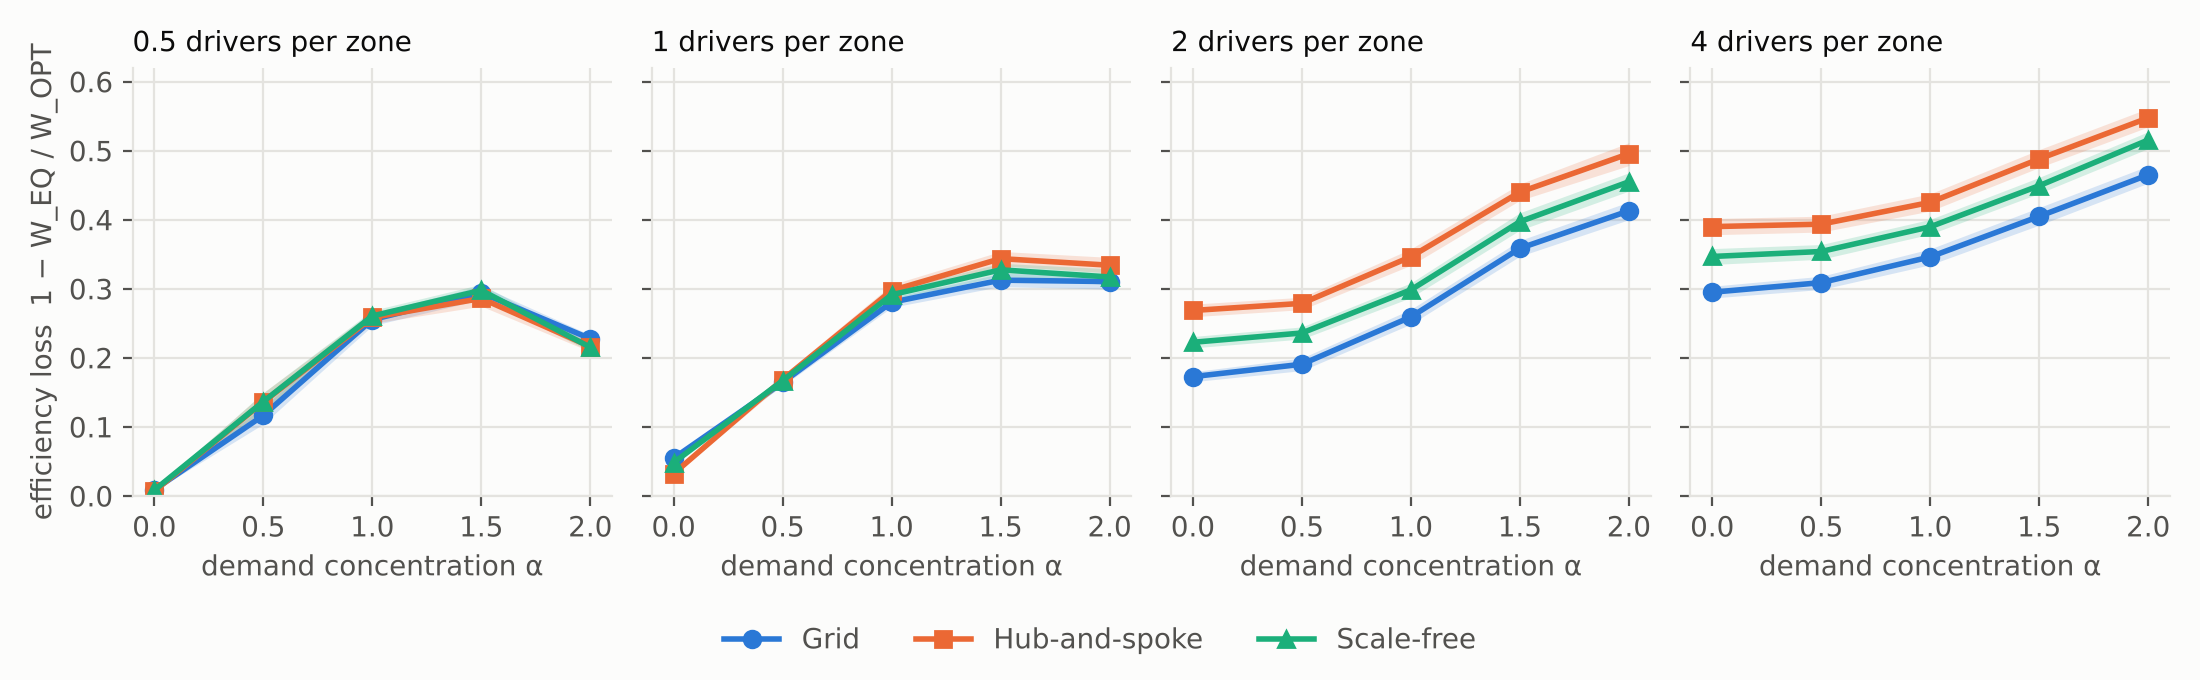
\includegraphics[width=\textwidth]{fig1_concentration.png}
\caption{Efficiency loss vs.\ demand concentration $\alpha$, one panel per driver density (100 seeds per point, bands: 95\% CI). Concentration and density raise the loss; topology separates only at $\rho\ge2$.}\label{fig:conc}\end{figure}
\textbf{H1 -- driver density: supported.} Mean loss rises from \lossRhoZeroPFive{} ($\rho=0.5$) to \lossRhoOnePZero{}, \lossRhoTwoPZero{} and \lossRhoFourPZero{} ($\rho=4$); $\rho$ explains \etaRho\% of the variance. \textbf{H2 -- demand concentration: supported, saturating.} Mean loss is \lossAlphaZeroPZero{}, \lossAlphaZeroPFive{}, \lossAlphaOnePZero{}, \lossAlphaOnePFive{}, \lossAlphaTwoPZero{} for $\alpha=0..2$ (\etaAlpha\% of the variance; Fig.~\ref{fig:conc}). At $\rho=0.5$ it is not monotone (peak \lowRhoPeak{} at $\alpha=\lowRhoPeakAlpha$, then \lowRhoLast{}): with few drivers the planner also sends everyone to the dominant zone. A linear model in topology, $H$, $\log_2\rho$ and $H\log_2\rho$ reaches $R^2=\olsRtwo{}$.
\textbf{H3 -- topology: weakly supported.} The ordering predicted in the idea review holds (grid \lossgrid{}, scale-free \lossscalefree{}, hub-and-spoke \losshubspoke{}) but topology explains only \etaTopo\% of the variance, and the gap vanishes unless drivers outnumber zones (Table~\ref{tab:topo}). Hubs funnel drivers through shared paths. When demand follows node degree, structure matters more (Table~\ref{tab:reg}).
\begin{table}[!ht]\centering\small
\begin{minipage}[t]{0.57\textwidth}\centering\scriptsize\tabTopoRho\captionof{table}{Efficiency loss by topology and density, mean $\pm$ 95\% CI half-width (all $\alpha$).}\label{tab:topo}\end{minipage}\hfill
\begin{minipage}[t]{0.40\textwidth}\centering\scriptsize\tabRegimes\captionof{table}{Loss by demand regime.}\label{tab:reg}\end{minipage}\end{table}

\begin{figure}[!ht]\centering
\begin{subfigure}{0.50\textwidth}\centering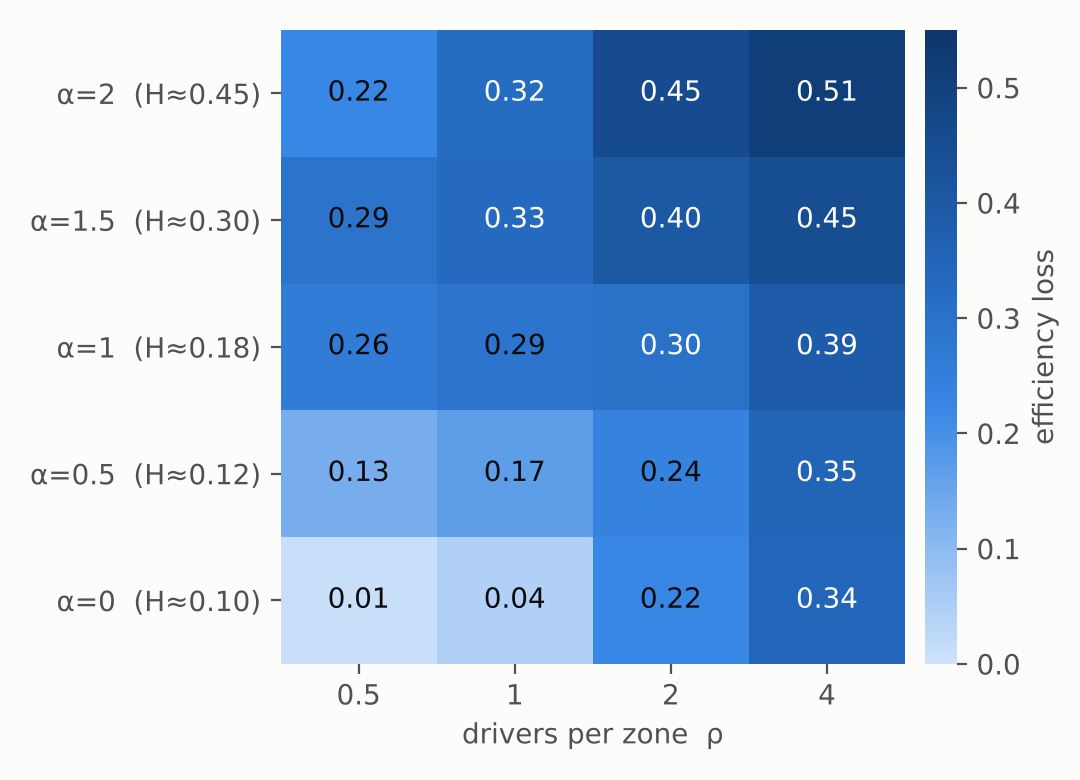
\includegraphics[width=\textwidth]{fig2_heatmap.png}\caption{Loss by $\alpha$ (with $H$) and $\rho$.}\end{subfigure}\hfill
\begin{subfigure}{0.48\textwidth}\centering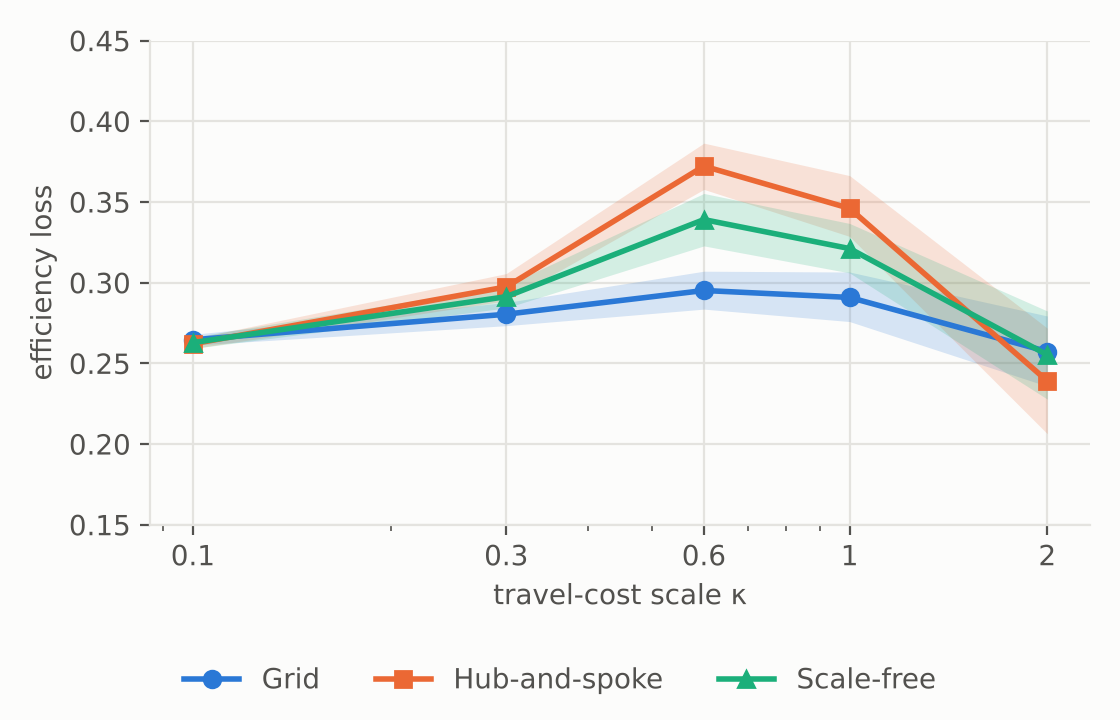
\includegraphics[width=\textwidth]{fig4_kappa.png}\caption{Loss vs.\ travel-cost scale $\kappa$.}\end{subfigure}
\caption{(a) Joint effect of concentration and density. (b) Travel cost: the loss peaks at $\kappa\approx\kapPeak{}$ (hub-and-spoke \kapHubAtPeak{}, grid \kapGridAtPeak{}) and falls at $\kappa=2$ ($\alpha=1,\rho=1$).}\label{fig:heat}\end{figure}
\textbf{H4 -- travel cost: non-monotone.} The loss rises from \kapLowEnd{} at $\kappa=0.1$ to a peak at $\kappa\approx\kapPeak{}$ and falls to \kapHighEnd{} at $\kappa=2$ (Fig.~\ref{fig:heat}b): when travel is expensive the optimum itself leaves most zones unserved and drivers idle, leaving less to coordinate.
Starting positions matter little: with a common depot the first-epoch costs are identical, every run reaches the same welfare (spread $\le$\depotSpread{}) and the loss is \startDepot{} against \startRandom{} with random starts.

\begin{figure}[!ht]\centering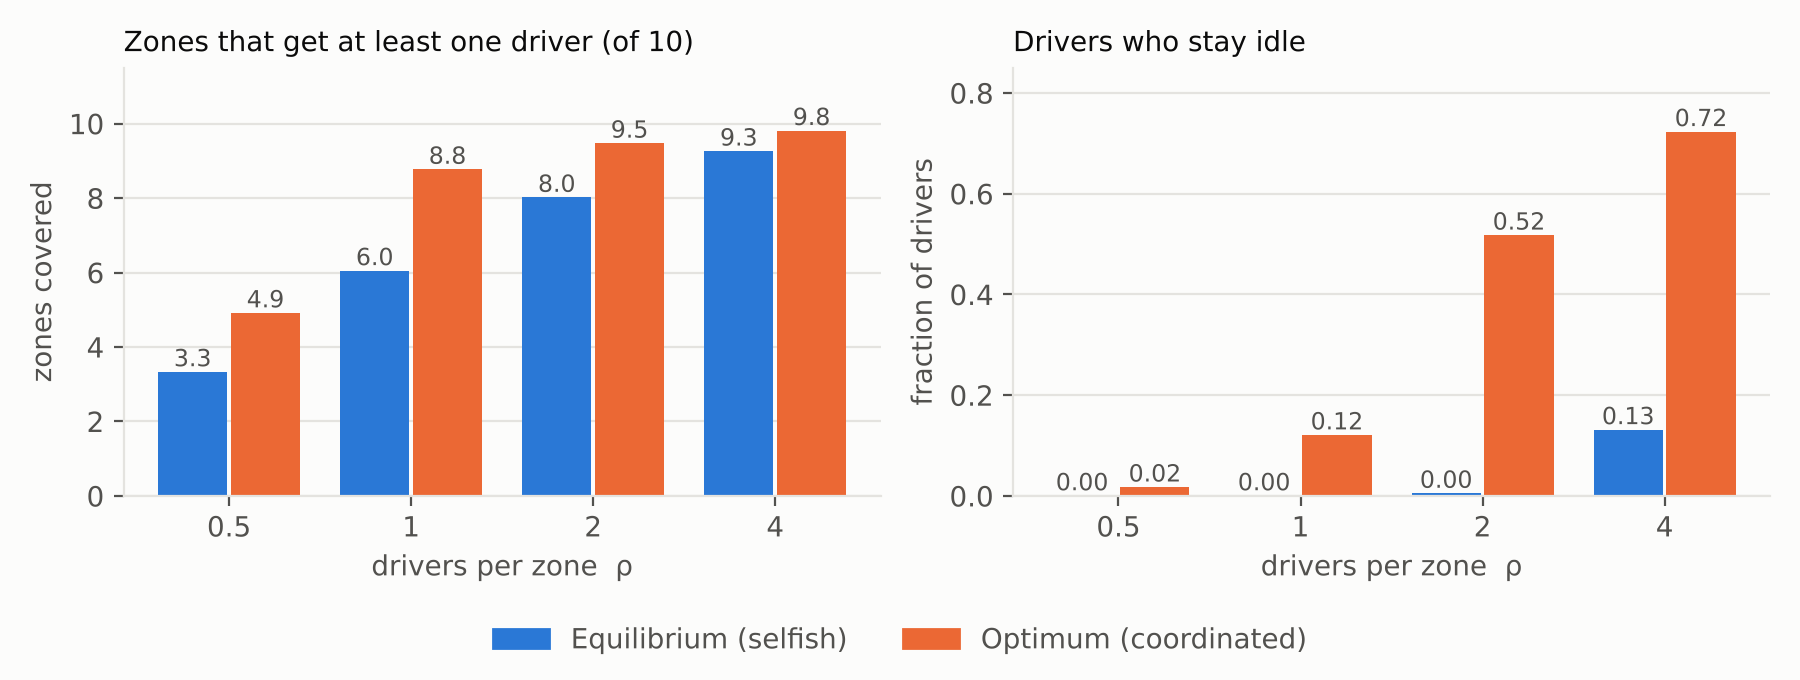
\includegraphics[width=0.92\textwidth]{fig3_coverage_idling.png}
\caption{Where the loss comes from: zones covered and idle drivers, equilibrium vs.\ optimum, by density.}\label{fig:cov}\end{figure}
\textbf{Mechanism.} Selfish drivers over-concentrate and over-enter (Fig.~\ref{fig:cov}). At $\alpha=2$ the busiest zone holds \eqMaxLoadAlphaTwo{} drivers at equilibrium against \optMaxLoadAlphaTwo{} at the optimum, and \eqCovAlphaTwo{} zones are covered against \optCovAlphaTwo{}. At $\rho=4$ the planner idles \optIdleRhoFour\% of drivers, selfish drivers only \eqIdleRhoFour\%: exactly the coverage externality of Sec.~\ref{sec:model}.

\begin{figure}[!ht]\centering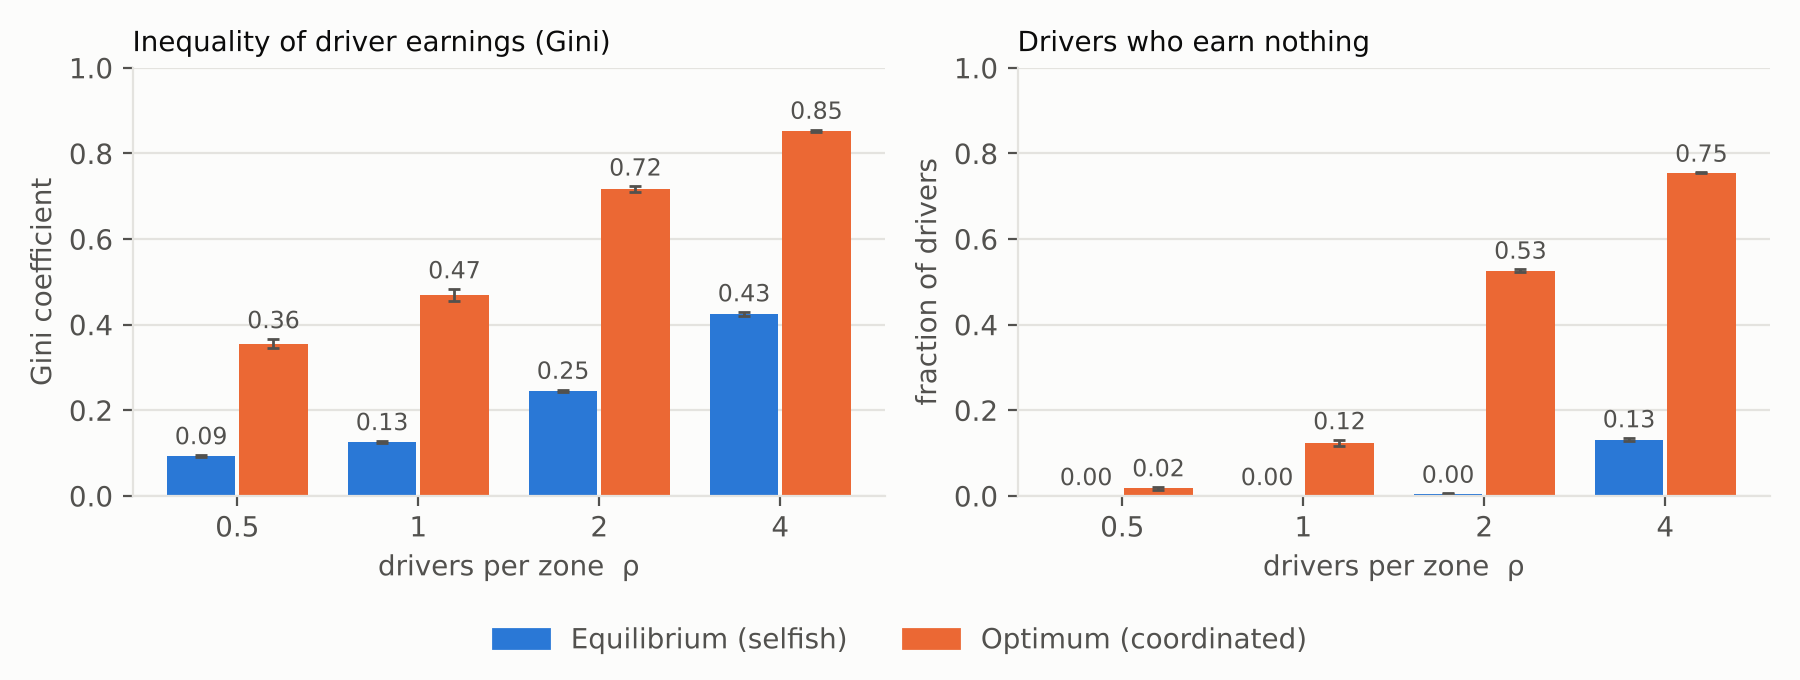
\includegraphics[width=0.6\textwidth]{fig6_equity.png}
\caption{Who earns what (experiment E; mean, 95\% CI). The more efficient optimum is far less equal: it idles surplus drivers, who earn nothing.}\label{fig:equity}\end{figure}
\textbf{Equity: is the optimum fairer?} The idea review asked whether the centralized optimum is efficient but inequitable. We replay the main sweep and record every driver's utility (no side payments: the planner decides who goes where, it does not redistribute fares). The Gini coefficient of driver utilities is \eGiniOptLow{} at the optimum against \eGiniEqLow{} at equilibrium for $\rho=0.5$, and \eGiniOptHigh{} against \eGiniEqHigh{} for $\rho=4$ (Fig.~\ref{fig:equity}); the optimum is the more unequal outcome in \eMoreUnequalSparse\% of instances with $\rho\le1$ and in \eMoreUnequalDense\% of those with $\rho\ge2$. The cause is the coverage externality again: with surplus drivers the planner keeps most of them idle (\eZeroOptHigh\% earn nothing at $\rho=4$, against \eZeroEqHigh\% at equilibrium), whereas selfish drivers all squeeze into zones and share. Efficiency and equity therefore pull apart; reconciling them needs transfers or rotating who idles across epochs, which the model excludes.
\textbf{Speed of convergence.} Best-response dynamics need about one profitable move per driver (\eUpdLow{} moves per driver at $\rho=0.5$ rising to \eUpdHigh{} at $\rho=4$; at most \eUpdMax{} in any instance) and \eSweepsLow{}--\eSweepsHigh{} round-robin sweeps on average, including the final sweep that confirms equilibrium (slowest instance \eSweepsMax{}); topology and concentration change this little.

\textbf{Learning unknown demand.} Fig.~\ref{fig:learn} and Table~\ref{tab:learn} give welfare relative to the full-information optimum.
\begin{figure}[!ht]\centering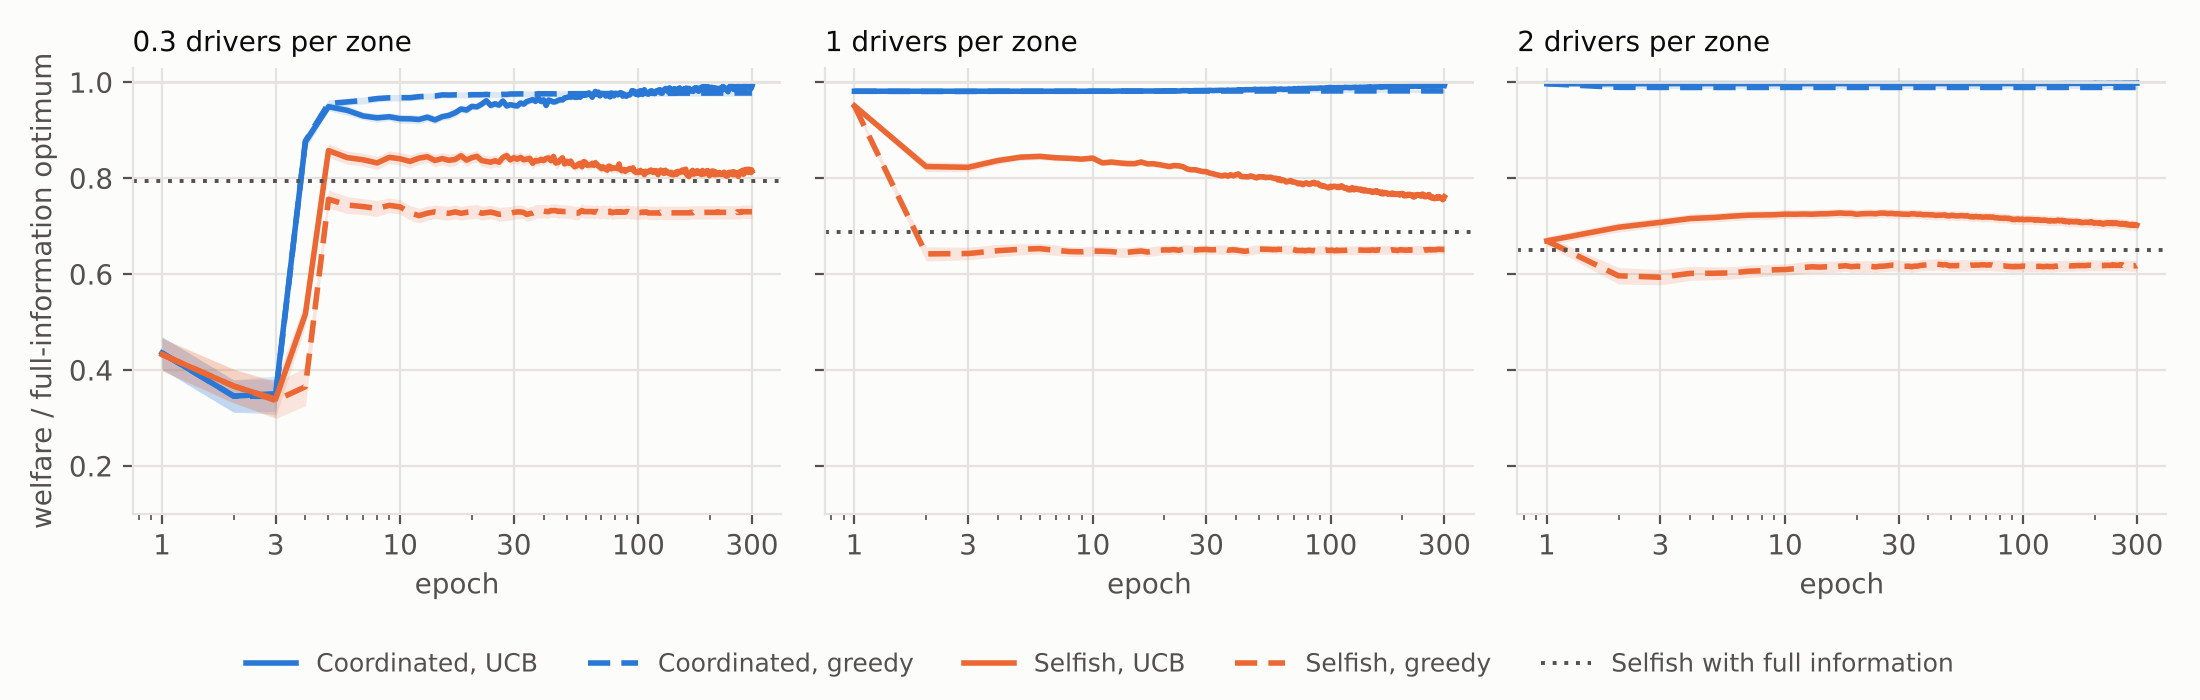
\includegraphics[width=\textwidth]{fig5_learning.png}
\caption{Learning curves (pooled over topologies and $\alpha$, 95\% CI). Coordinated agents reach near-optimal welfare within a few epochs; selfish agents plateau at the equilibrium level.}\label{fig:learn}\end{figure}
\begin{table}[!ht]\centering\small\tabLearning\caption{Efficiency (welfare / full-information optimum), epochs 151--300.}\label{tab:learn}\end{table}
\emph{Learning is cheap, selfishness is not.} The coordinated dispatcher reaches at least \lrnPlanMin{} of the optimum and loses the equivalent of \lrnPlanCumMin{}--\lrnPlanCumMax{} full-welfare epochs out of 300 (under 3\%); the only visible cost is at $\rho=0.3$, where three drivers serve ten zones and each visit is exploration. Selfish drivers lose \lrnSelfCumUMin{}--\lrnSelfCumUMax{} epochs with UCB and \lrnSelfCumGMin{}--\lrnSelfCumGMax{} with greedy beliefs, almost all of it the price of anarchy rather than ignorance (with $\rho\ge1$ the optimism of epoch 1 already covers every zone, so exploration is free).
\emph{The exploration bonus acts as a subsidy.} Selfish agents with UCB beliefs are \emph{more} efficient than selfish agents who know the demand, in \lrnUcbBeatsFI\% of instances (mean \lrnUcbGain{}; \lrnRhoOneUcb{} vs.\ \lrnRhoOneFI{} at $\rho=1$), greedy ones less so (\lrnGreedyGain{}). The bonus inflates rarely served zones and moves drivers off the hotspots, partly offsetting the externality. It fades slowly: in a 6{,}000-epoch run at $\rho=1$ (\lhN{} seeds) efficiency is \lhFirst{}, \lhMid{} and \lhLast{} over epochs 1--50, 250--350 and 5500--6000, still \lhGain{} above the full-information equilibrium (\lhFI{}). Drivers act on inflated beliefs, so this is an observation about the externality, not a policy.

\section{Discussion, Limitations and Future Work}\label{sec:disc}
\textbf{Findings.} (i) The loss of selfish positioning is governed by how many drivers compete for how concentrated a demand, not by street layout; (ii) it is caused by a precise externality, which also explains why the optimum idles drivers; (iii) not knowing demand is a second-order cost compared with selfishness. \textbf{Limitations.} Demand is static and shared equally with no capacity limit; the city is stylized, not calibrated on real data, so absolute losses describe the model, not a real city; equilibrium selection is sampled (not worst-case) when instances are too large to enumerate; learning uses pooled beliefs. \textbf{Future work.} (1) \emph{Cooperation that is not free}: enforcing the coordinated outcome needs penalties or incentives, e.g.\ a toll on joining an occupied zone, and information may be costly; (2) \emph{cliques} of drivers who coordinate among themselves but not with the rest; (3) time-varying demand and capacity limits; (4) calibrating topologies and demand on real cities.

\section{Contributions}\label{sec:contrib}
\begin{table}[!ht]\centering\footnotesize
\begin{tabular}{p{2.1cm}p{5.6cm}p{7.0cm}}\toprule \textbf{Member} & \textbf{Assigned task} & \textbf{Status}\\\midrule
Jahanzaib & Game formulation, utility function and its justification, potential-game analysis, best-response simulator, equilibrium enumeration, learning extension, experiments and analysis, report & Fulfilled: all items implemented, tested and used for the results above. \confirm{[confirm/adjust]}\\
Mukkesh Dudekula & City generators (grid, hub-and-spoke, scale-free), edge weights, shortest paths & Fulfilled: module delivered with 77 passing tests; used unchanged for all experiments\\
Thushar Vunnam & Demand generators and the centralized optimizer (exact, integer program, local search) & Fulfilled after one fix: 58 of 59 tests passed on delivery; the integer program missed the zone-activation constraint (patched and covered by a regression test, Sec.~\ref{sec:verify}). Demand generators used unchanged\\
Lohith & Experiment sweeps, aggregation, plots, experimental sections of the report & Experiment sweeps V, A, B, C, D, L; bootstrap aggregation and variance decomposition; all figures; the generated numbers and tables (\texttt{make\_tables.py}); the results section. Added experiment E (equity and convergence speed), the two idea-review metrics not reported before. All sweeps rerun bit-for-bit from fixed seeds. \confirm{[confirm/adjust]}\\\bottomrule
\end{tabular}\caption{Contributions.}\end{table}

\section{Reproducibility}\label{sec:repro}
Repository: \confirm{[insert link]}. \texttt{bash run\_all.sh} runs the tests, all sweeps (fixed seeds), the analysis, the figures and rebuilds this report from the CSVs; the README maps every figure and table to the script that produces it.
\begin{thebibliography}{9}\footnotesize
\bibitem{ros73} R.~W.~Rosenthal. A class of games possessing pure-strategy Nash equilibria. \emph{Int.\ J.\ Game Theory}, 2:65--67, 1973.
\bibitem{mil96} I.~Milchtaich. Congestion games with player-specific payoff functions. \emph{Games and Economic Behavior}, 13(1):111--124, 1996.
\bibitem{mon96} D.~Monderer and L.~S.~Shapley. Potential games. \emph{Games and Economic Behavior}, 14(1):124--143, 1996.
\bibitem{kp99} E.~Koutsoupias and C.~Papadimitriou. Worst-case equilibria. \emph{STACS}, 1999.
\bibitem{auer02} P.~Auer, N.~Cesa-Bianchi and P.~Fischer. Finite-time analysis of the multiarmed bandit problem. \emph{Machine Learning}, 47:235--256, 2002.
\end{thebibliography}
\end{document}
